\documentclass[a4paper, 12pt]{article}

\usepackage{wrapfig}
\usepackage{graphicx}
\usepackage{mathtext}
\usepackage{amsmath}
\usepackage{siunitx}
\usepackage{multirow}
\usepackage{rotating}
\usepackage{float}

\usepackage[T1,T2A]{fontenc}

\usepackage[russian]{babel}
\usepackage{amsfonts} 
\graphicspath{{pictures/}}
\usepackage[a4paper,left=25mm,right=25mm,top=20mm,bottom=20mm]{geometry} % устанавливает поля документа

\title{\begin{center}Лабораторная работа №1.4.8\end{center}
Измерение модуля Юнга методом акустического резонанса}
\author{Каспаров Н.М.}
\date{\today}

\begin{document}
    \pagenumbering{gobble}
    \maketitle
    \newpage
    \pagenumbering{arabic}
    
    \section{Цель работы}
    \begin{enumerate}
        \item Исследовать явление акустического резонанса в тонком стержне.
        \item Измерить скорость распространения продольных звуковых колебаний в тонких стержнях из различных материалов и различных размеров.
        \item Измерить модули Юнга различных материалов.
    \end{enumerate}
    
    \section{В работе используется}
    \begin{enumerate}
        \item Генератор звуковых частот.
        \item Частотомер.
        \item Осциллограф.
        \item Электромагнитные излучатель и приёмник колебаний.
        \item Набор стержней из различных материалов.
        \item Линейка, штангенциркуль, микрометр.
        \item Весы.
    \end{enumerate}

    \section{Введение}
        Акустическая волна, распространяющаяся в стержне конечной длины $L$,
        испытает отражение от торцов стержня. Если при этом на длине стержня
        укладывается целое число полуволн, то отражённые волны будут складываться в фазе с падающими, что приведёт к резкому усилению амплитуды
        их колебаний и возникновению акустического резонанса в стержне. Измеряя соответствующие резонансные частоты, можно определить скорость
        звуковой волны в стержне и, таким образом, измерить модуль Юнга материала стержня. Акустический метод является одним из наиболее точных
        методов определения упругих характеристик твёрдых тел.
    \section{Уравнение волны в тонком стержне}
    \begin{minipage}{0.6\textwidth}
        Направим ось $X$ вдоль геометрической оси стержня (рис. 1). Разобьём
        исходно недеформированный стержень на тонкие слои толщиной $\Delta x$. При
        продольной деформации среды границы слоёв сместятся в некоторые новые положения. Пусть плоскость среды, находящаяся исходно в точке $x$,
        сместилась к моменту $t$ на расстояние $\xi(x,t)$. Тогда слой, занимавший исходно отрезок $[x; x + \Delta x]$, изменил свой продольный размер на величину $\Delta \xi = \xi(x + \Delta x, t) - \xi(x, t)$.
    \end{minipage}
    \hfill
    \begin{minipage}{0.35\textwidth}
        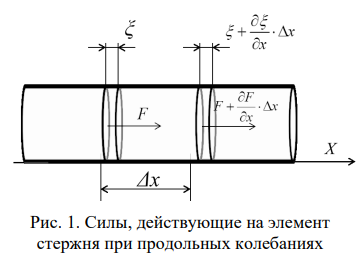
\includegraphics[scale=0.7]{picture1.png}
    \end{minipage}
        
        \begin{equation}
            \varepsilon = \frac{\partial\xi}{\partial x}
        \end{equation}

        Далее, согласно закону Гука, имеем:
        
        \begin{equation}
            \sigma = \varepsilon E = E \frac{\partial\xi}{\partial x}
        \end{equation}
        
        Здесь напряжение равно $\sigma = \frac{F}{S}$, где 
        
        $F$ — продольная сила, действующая на элементарный участок $\Delta x$, 
        
        $S$ - площадь поперечного сечения стержня. 

        Напряжения, действующие на стенки рассматриваемого элемента в сечениях $x$ и $x + \Delta x$, будут различными. Из-за этого возникнет результирующая возвращающая сила, стремящаяся вернуть элемент стержня в исходное (недеформированное и несмещённое) состояние:
        \begin{equation}
            \Delta F = S \sigma(x + \Delta x) - S \sigma(x) = \frac{\partial\sigma}{\partial x} S\Delta x = \frac{\partial^2\xi}{\partial^2 x} ES\Delta x
        \end{equation}

        Эта сила вызовет ускорение движение элемента стержня массой $\Delta m = S \rho \Delta x$ вдоль оси $X$. Ускорение рассматриваемого элемента — это вторая производная по времени от смещения его границ:
        \begin{equation}
            a = \frac{\partial^2 \xi}{\partial t^2}
        \end{equation}

        Тогда, используя 2-й закон Ньютона:
        \begin{equation}
            \Delta m \cdot a = \Delta F
        \end{equation}

        и соотношения (1) - (4), получим уравнение движения среды:

        \begin{equation}
            S \rho \Delta x \frac{\partial^2 \xi}{\partial t^2} = ES\Delta x \frac{\partial^2\xi}{\partial^2 x}
        \end{equation}

        Cкорость $u$ распространения продольной акустической волны в простейшем случае длинного тонкого стержня определяется соотношением:
        \begin{equation}
            u = \sqrt{\frac{E}{\rho}}
        \end{equation}

        Теперь, используя соотношения (6) - (7), мы можем записать волновое уравнение:
        \begin{equation}
            \frac{\partial^2 \xi}{\partial t^2} = u^2 \frac{\partial^2\xi}{\partial^2 x}
        \end{equation}
        
        Оно имеет универсальный характер и описывает волны самой разной природы: акустические волны в твёрдых телах, жидкостях и газа, волны на струне, электромагнитные волны и т.п. Величина $u$ в уравнении (6) имеет смысл скорости распространения волны.

    \section{Собственные колебания стержня. Стоячие волны}
        В случае гармонического возбуждения колебаний с частотой $f$ продольная волна в тонком стержне может быть представлена в виде суперпозиции двух бегущих навстречу гармонических волн:

        \begin{equation}
            \xi(x, t) = A_1 (\sin{\omega t - kx + \phi_1}) + A_2 (\sin{\omega t - kx + \phi_2}),
        \end{equation}
        где $\omega = 2 \pi f$ — циклическая частота. Коэффициент $k = \frac{2 \pi}{\lambda}$ называют
        волновым числом или пространственной частотой волны.
        
        Пусть концы стержня не закреплены. Тогда напряжения в них должны равняться нулю. Положим координаты торцов равными $x = 0$ и $x = L$. Тогда, используя связь напряжения и деформации (2), запишем граничные условия для свободных (незакреплённых) концов стержня:

        \begin{equation}
            x = 0: \sigma(0) = 0 \rightarrow \frac{\partial\xi}{\partial x} = 0
        \end{equation}
        \begin{equation}
            x = L: \sigma(L) = 0 \rightarrow \frac{\partial\xi}{\partial x} = 0
        \end{equation}

        Нетрудно видеть, что это соотношение будет выполняться при любом $t$, если только у «падающей» и «отражённой» волн одинаковы амплитуды 

        \begin{equation}
            A_1 = A_2
        \end{equation}
        и фазы.
        \begin{equation}
            \phi_1 = \phi_2
        \end{equation}
        
        Далее, перепишем исследуемую функцию (9), используя граничные условия (12) и (13) и формулу суммы синусов:

        \begin{equation}
            \xi(x, t) = 2A \cos(kx)sin(\omega t + \phi)
        \end{equation}

        Колебания вида (14) называют гармоническими стоячими волнами.

        Наконец, воспользуемся вторым граничным условием (9) применительно к функции (12). В результате придём к уравнению $\sin(kL) = 0$, решения которого определяют набор допустимых значений волновых чисел $k$:

        \begin{equation}
            k_n L = \pi n, \quad n = 1, 2, 3,...,
        \end{equation}
        
        или, выражая (13) через длину волны $\lambda = \frac{2 \pi}{k},$, получим

        \begin{equation}
            \lambda_n = \frac{2L}{n}, \quad n \in \mathbb{N}
        \end{equation}
        Таким образом, для возбуждения стоячей волны на длине стержня должно укладываться целое число полуволн.
        
        Допустимые значения частот:
        \begin{equation}
            f_n = \frac{u}{\lambda_n} = n \frac{u}{2L}, \quad n \in \mathbb{N}
        \end{equation}
        называют собственными частотами колебаний стержня длиной $L$. Именно при совпадении внешней частоты с одной из частот $f_n$ в стержне возникает акустический резонанс.
        
        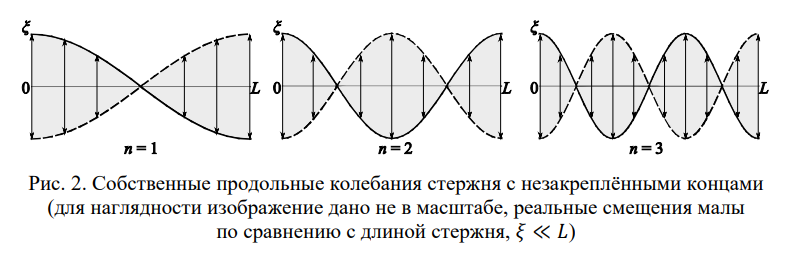
\includegraphics[scale=0.75]{picture2.png}
        Зависимость амплитуды смещения от координаты для собственных колебаний стержня с незакреплёнными концами при $n = 1,2,3$ представлена на рис. 2. 

    \section{Схема}

    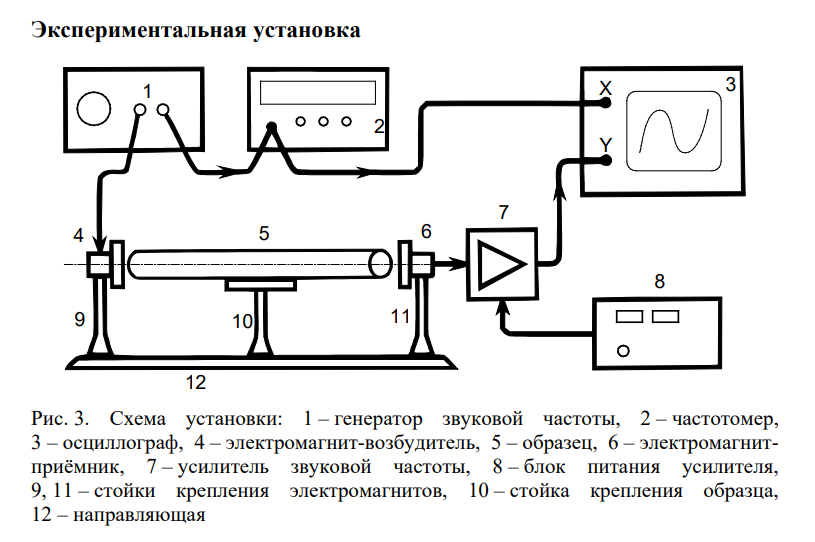
\includegraphics[scale=0.75]{picture3.png}
    
    Схема экспериментальной установки приведена на рис. 3. Исследуемый
    стержень \textbf{5} размещается на стойке \textbf{10}. Возбуждение и приём колебаний в
    стержне осуществляются электромагнитными преобразователями \textbf{4} и \textbf{6},
    расположенными рядом с торцами стержня. Крепления \textbf{9}, \textbf{11} электромагнитов дают  возможность регулировать их расположение по высоте, а
    также перемещать вправо-влево по столу \textbf{12}.

    Электромагнит \textbf{4} служит для возбуждения упругих механических продольных колебаний в стержне. На него с генератора звуковой частоты \textbf{1} подаётся сигнал синусоидальной формы: протекающий в катушке электромагнита ток создаёт пропорциональное ему магнитное поле, вызывающее периодическое воздействие заданной частоты на торец стержня (к торцам
    стержней из немагнитных материалов прикреплены тонкие стальные
    шайбы). Рядом с другим торцом стержня находится аналогичный электромагнитный датчик \textbf{6}, который служит для преобразования механических
    колебаний в электрические. Принцип работы электромагнитных датчиков
    описан подробнее ниже.

    Сигнал с выхода генератора поступает на частотомер \textbf{2} и на вход
    канала \textbf{X} осциллографа \textbf{3}. ЭДС, возбуждаемая в регистрирующем электромагните \textbf{6}, пропорциональная амплитуде колебаний торца стержня, усиливается усилителем \textbf{7} и подаётся на вход канала \textbf{Y} осциллографа.

    Изменяя частоту генератора и наблюдая за амплитудой сигнала с регистрирующего датчика, можно определить частоту акустического резонанса в стержне. Наблюдения в режиме \textbf{X}–\textbf{Y} позволяют сравнить сигналы генератора и датчика, а также облегчает поиск резонанса при слабом сигнале.
    \newpage
    \section{Ход работы}
    \subsection{Измерение геометрических параметров стержня}

    Используя металлическую линейку и микрометр измерим длину и диаметр данных стержней. Для измерения диаметра проведем множество измерений на всей протяженности стержня. Занесем данные в таблицу 1.
    
    \begin{table}[h]
        \centering
        \begin{tabular}{|c|c|c|c|c|c|c|}
            \hline
             &
              \multicolumn{1}{c|}{$l$, см} &
              \multicolumn{1}{c|}{$\sigma_l$, см} &
              \multicolumn{1}{c|}{$\varepsilon_l$} &
              \multicolumn{1}{c|}{$d$, мм} &
              \multicolumn{1}{c|}{$\sigma_d$, мм} &
              \multicolumn{1}{c|}{$\varepsilon_d$} \\ \hline
            Медь   & 60.5 & 0.1 & $2 \cdot 10^{-3}$ & 11.96 & 0.01 & $8 \cdot 10^{-4}$ \\ \hline
            Сталь  & 60.4 & 0.1 & $2 \cdot 10^{-3}$ & 11.98 & 0.01 & $8 \cdot 10^{-4}$ \\ \hline
            Дюраль & 60.5 & 0.1 & $2 \cdot 10^{-3}$ & 12.23 & 0.01 & $8 \cdot 10^{-4}$ \\ \hline
        \end{tabular}
        \caption{Измерения геометрических показателей стержней}
    \end{table}

    Заметим, что действительно $\frac{R}{d} \ll 1$, значит стержень можно назвать тонким.
    
    Все измерения диаметра дали одинаковые результаты, поэтому будем считать диаметр стержней постоянным.

    \subsection{Измерение плотности материалов}

    Используя штангенциркуль и микрометр, определим геометрические параметры цилиндрических образцов, а с помощью весов определим массу. Занесем данные в таблицу 2.

    \begin{table}[h]
        \centering
        \begin{tabular}{|c|c|c|c|c|c|c|c|c|c|}
        \hline
         & $l$, мм & $\sigma_l$, мм & $\varepsilon_l$ & $d$, мм & $\sigma_d$, мм & $\varepsilon_d$ & $m$, гр & $\sigma_m$, гр & $\varepsilon_m$ \\ \hline
        Медь   & 30.05 & 0.05 & $2 \cdot 10^{-3}$ & 11.85 & 0.01 & $8\cdot 10^{-4}$ & 29.450 & 0.001 & $3\cdot 10^{-5}$ \\ \hline
        Сталь  & 40.00 & 0.05 & $1 \cdot 10^{-3}$ & 11.99 & 0.01 & $8\cdot 10^{-4}$ & 35.185 & 0.001 & $3\cdot 10^{-5}$ \\ \hline
        Дюраль & 30.00 & 0.05 & $2 \cdot 10^{-3}$ & 12.04 & 0.01 & $8\cdot 10^{-4}$ &  9.484 & 0.001 & $1\cdot 10^{-5}$ \\ \hline
        \end{tabular}
        \caption{Измерения для определения плотности образцов}
    \end{table}

    Чтобы найти плотность материала, воспользуемся формулой:

    \begin{equation}
        \rho = \frac{4m}{\pi d^2 \cdot l}
    \end{equation}

    Погрешностью $\varepsilon_m$ можно пренебречь. Учитывая это, формула для рассчета погрешности измерения плотности:

    \begin{equation}
        \varepsilon_q = \sqrt{(\frac{\sigma_l}{l})^2 + (2\frac{\sigma_d}{d})^2}
    \end{equation}

    Проведем расчет и занесем результаты в таблицу 3.
    \begin{table}[h]
    \centering
        \begin{tabular}{|c|c|c|c|}
        \hline
        \multicolumn{1}{|l|}{} & $\rho$, $гр/см^3$ & $\sigma_{\rho}$, $гр/см^3$ & $\varepsilon_{\rho}$ \\ \hline
        Медь                   & 8.89         & 0.02               & $2 \cdot 10^{-3}$       \\ \hline
        Сталь                  & 7.79         & 0.02               & $2 \cdot 10^{-3}$       \\ \hline
        Дюраль              & 2.78         & 0.01               & $2 \cdot 10^{-3}$       \\ \hline
        \end{tabular}
        \caption{Результаты расчета плотности материалов}
    \end{table}

\newpage

    \subsection{Измерение резонансных частот стержней}

    Будем менять частоту генератора в пределах ожидаемых значений резонанса. Оценить её можно по формуле
    \begin{equation}
        f_1 = \frac{u}{2L},
    \end{equation}
    воспользовавшись табличным значением скорости продольных волн.
    
    После нахождения значения первого резонанса, умножим его на $n$ и уже в новой окресности ищем значения $n$-ной резонансной частоты. 
    
    Результаты внесем в таблицу 4:

    \begin{table}[h]
    \centering
    \begin{tabular}{|c|ccc|}
    \hline
    n & \multicolumn{1}{c|}{Медь}   & \multicolumn{1}{c|}{Сталь}  & Дюраль \\ \hline
    1 & \multicolumn{1}{c|}{32,501} & \multicolumn{1}{c|}{41,277} & 42,498 \\ \hline
    2 & \multicolumn{1}{c|}{65,002} & \multicolumn{1}{c|}{82,504} & 84,995 \\ \hline
    3 & \multicolumn{1}{c|}{97,516} & \multicolumn{1}{c|}{124,01} & 127,64 \\ \hline
    4 & \multicolumn{1}{c|}{130,02} & \multicolumn{1}{c|}{165,20}  & 170,3  \\ \hline
    5 & \multicolumn{1}{c|}{162,19} & \multicolumn{1}{c|}{206,52} & 212,82 \\ \hline
    6 & \multicolumn{1}{c|}{194,87} & \multicolumn{1}{c|}{247,73} & 255    \\ \hline
    7 & \multicolumn{1}{c|}{226,83} & \multicolumn{1}{c|}{289,12} & 297,26 \\ \hline
      & \multicolumn{3}{c|}{$f_n, 10^2 \cdot Гц$}                                  \\ \hline
    \end{tabular}
    \caption{Результаты измерения резонантных частот стержней}
    \end{table}

    Представим результаты в виде графика $f_n(n)$ и убедимся, что получатся прямые, проходящие через начало координат ($f_n = f_1 \cdot n$) (рис. 1)
    \begin{figure}[h]
        \centering
        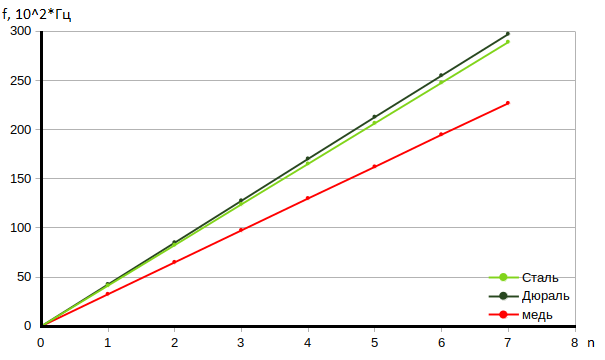
\includegraphics[scale=1.00]{graph.png}
        \caption{График зависимости $f_n(n)$}
        \label{fig:enter-label}
    \end{figure}

    Найдём $f_1$ по формуле:

    \begin{equation}
		k=\frac{\langle xy\rangle-\langle x\rangle \langle y\rangle}{\langle x^2\rangle - \langle x\rangle^2}
	\end{equation}

    Систематическая погрешность мала по сравнению со случайной, поэтому ей можно пренебречь.

    Значит, погрешность будет определяться случайной составляющей. Найдем её по формуле:

	\begin{equation}
		\sigma_k=\sigma_k^\text{случ}=\frac{1}{\sqrt{N}}\sqrt{\frac{\langle y^2 \rangle - \langle y \rangle^2}{\langle x^2 \rangle - \langle x \rangle^2} - k^2  }
	\end{equation}
    
    Результаты занесём в таблицу 5:

    \begin{table}[h]
    \centering
        \begin{tabular}{|c|c|c|c|}
        \hline
        \multicolumn{1}{|l|}{} & Медь  & Сталь & Дюраль \\ \hline
        $f_1$, Гц              & 3241  & 4130  & 4248   \\ \hline
        $\sigma_{f_1}$, Гц     & 3     & 1     & 3      \\ \hline
        $\varepsilon_{f_1}$    & $9\cdot 10^{-4}$ & $2\cdot 10^{-4}$ & $7\cdot 10^{-4}$  \\ \hline
        \end{tabular}
        \caption{Результаты расчета первой резонантной частотой}
    \end{table}

    \subsection{Расчет скорости продольных волн в тонком стержне}

    Рассчитаем скорость звука $u$ в тонких стержнях. 
    
    Из формулы (20) получим:

    \begin{equation}
        u = 2f_1L
    \end{equation}

    Погрешность найдем по соотношению:

    \begin{equation}
        \varepsilon_u = \sqrt{(\frac{\sigma_{f_1}}{f_1})^2 + (\frac{\sigma_L}{L})^2}
    \end{equation}

    Данные внесем в таблицу:

    \begin{table}[h]
    \centering
        \begin{tabular}{|c|c|c|c|}
        \hline
        \multicolumn{1}{|l|}{} & Медь  & Сталь & Дюраль \\ \hline
        $u,$ м/c               & 3922  & 4989  & 5140   \\ \hline
        $\sigma_u$, м/c        & 7     & 8     & 9      \\ \hline
        $\varepsilon_u$,       & $2\cdot 10^{-3}$ & $2\cdot 10^{-3}$ & $2\cdot 10^{-3}$  \\ \hline
        \end{tabular}
        \caption{Результаты расчета скорости звука в тонких стержнях}
    \end{table}

    \subsection{Расчет модуля Юнга различных материалов}

    Найдем модуль Юнга материалов стержней. Сравним их с табличными данными.

    Из формулы (7) выразим модуль Юнга $E$:

    \begin{equation}
        E = \rho * u^2
    \end{equation}

    Погрешность модуля Юнга можно посчитать по данной формуле:

    \begin{equation}
        \varepsilon = \sqrt{\varepsilon_{\rho}^2 + 4\varepsilon_u^2}
    \end{equation}

    \newpage
    
    Результаты расчета представим в таблице 7:

    \begin{table}[h]
    \centering
        \begin{tabular}{|c|c|c|c|}
        \hline
        \multicolumn{1}{|l|}{} & Медь  & Сталь & Дюраль \\ \hline
        $E$, ГПа               & 137   & 194   & 73     \\ \hline
        $\sigma_E$, ГПа        & 7     & 9     & 4      \\ \hline
        $\varepsilon_u$, \%    & 5     & 5     & 5      \\ \hline \hline
        $E_{\text{табл}}$, ГПа & 129   & 200   & 74     \\ \hline
        \end{tabular}
        \caption{Результаты расчета модуля Юнга и их табличные значения.}
    \end{table}

    Как мы видим, значения совпали в пределах погрешности.

    \section{Вывод}

    В данной работе мы экспериментально показали, что отношение резонантной частоты к номеру гармоники $f_n/n$ остается постоянным. Мы также вычислили значения скорости продольных волн в тонких стержнях, провели расчеты модуля Юнга для меди, стали и дюралюминия, которые совпали с табличными значениями в пределах погрешности:

    $$E_м = (137 \pm 7) ГПа$$
    $$E_с = (194 \pm 9) ГПа$$
    $$E_д = (73 \pm 4) ГПа$$

    Для дальнейшего повышения точности измерений, необходимо увеличить точность измерения длин стержней, поскольку погрешность в их измерении в значительной степени определяет окончательные погрешности.
    
\end{document}